\begin{frame}
\frametitle{Problem Statement-Quadrilateral Construction}
\begin{enumerate}[label=(\roman*)]
\item Construct DEAR with DE = 4, EA = 5, AR = 4.5, $\angle {E}$ = 60$\degree$ and $\angle {A}$ = 90$\degree$.\\
\textbf{Soln:}\\
Given:-  DE = 4, EA = 5, AR = 4.5, $\angle {E}$ = 60$\degree$ and $\angle {A}$ = 90$\degree$\\
  \end{enumerate}
\url{https://github.com/Rajolep/_Geometry/blob/master/codes/Quad/drawquad.py}
\begin{figure}
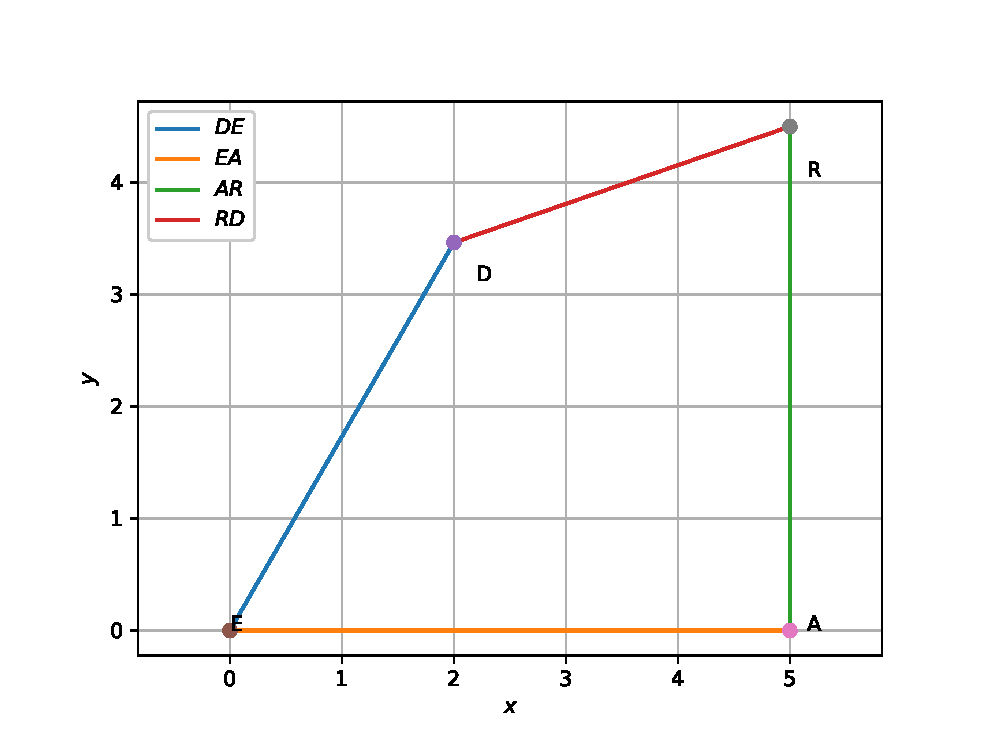
\includegraphics[scale=0.4]{./figs/quadcon.eps}
\end{figure}
\end{frame}
\begin{frame}
\begin{figure}
origin/E(0,0)
\begin{tikzpicture}
[scale =0.9,>=stealth,point/.style = {draw, circle, fill = black, inner sep = 1pt},]
\node (D) at (2,3.464)[point,label=above :$D$] {};
\node (E) at (0,0)[point,label=below :$E$] {};
\node (A) at (5,0)[point,label=below :$A$] {};
\node (R) at (5,4.5)[point,label=above :$R$] {};
\draw (D)--(E);
\draw (E)--(A);
\draw (A)--(R);
\draw (R)--(D);
\tkzMarkAngle[fill=white!60,size=.3](A,E,D)
\tkzLabelAngle[pos=0.65](A,E,D){$60$}
\tkzMarkRightAngle[draw=black,size=.2](R,A,E)
\end{tikzpicture}

\end{figure}
\url{https://github.com/Rajolep/_Geometry/blob/master/figs/quadccon.tex}
\end{frame}
\begin{frame}
Construction steps:
\begin{itemize}
\item E(0,0)  A(4,0) R(4,5)
\item step1 : From given draw the line segments
\item step2 : draw a line segment/diagnol and calculate its value \\
    p=$\sqrt{(EA)^2(AR)^2-2(EA)(AR)\cos{60}}$\\
     by using cosine formula,\\
 \item step3 : coordinates of D(x,y)   \\x=$\frac{(c)^2+(b)^2-(p)^2}{2c}$ y=$\sqrt{(b)^2-(x)^2}$   \\
     D(2,3.46)
     
\end{itemize}
\end{frame}
